\chapter{Implementation and Results}
\label{Chapter5} 


This chapter allows us to present the achieved work. We begin by listing the technologies and the software environment used throughout the project life cycle. After that, we present an overview of the achieved results and screenshots from different interfaces of our application. We end up this chapter with showing the flowed time-line during our project. 



\section{Implementation Environment}
\subsection{Hardware Tools}
To achieve this work we used a personal computer with the following characteristics:\\	

{\bf Workstation :}\\
Band: Laptop HP Probook 450 g3\\
Processor: Intel Core i7 CPU\\
Memory: 8,00GO of RAM\\
Operating system: Windows 10.


\subsection{Software Tools}

To achieve this work, we used  the software mentioned in the table \ref{sf}. More details in appendix A.
\begin{table}[!h]
\caption{Software Environment Characteristics}
\begin{center}
\begin{tabularx}{17cm}{ |p{4cm}|X|X| } 
 \hline
 \textbf{Tool} & \textbf{Category} & \textbf{Usage} \\ \hline
 Visual Studio 2012 Ultimate & Integrated Development Environment (IDE) & Developing the web controls.\\ \hline
Microsoft SQL Server & Database management system & Manage user information and users' accounts\\ \hline
Spyder & Integrated Development Environment (IDE) & Developing the service controllers.\\ \hline
Anaconda & Anaconda is a freemium open source distribution of the Python programming languages & Build the service.\\ \hline
Microsoft Project & Project Management Software & Developing plans and tracking progress. \\ \hline
\end{tabularx}
\end{center}
\label{sf}
\end{table}
\subsection{Technological Choices}
The table \ref{ut} shows the list of the used technologies. More details in appendix A.
\begin{table}[!h]
\caption{Used Technologies}
\begin{center}
\begin{tabularx}{17cm}{ |p{3cm}|X| } 
 \hline
 \textbf{Technology} & \textbf{Usage}  \\ \hline
 
C\# & The main programming language used for the code behind web pages.\\ \hline
ASP.Net & The used framework for developing the web controls. \\ \hline
DevExpress & The used library to design charts.\\ \hline
Python & The used programming language for implementing the service.\\ \hline
Apache Spark & Framework for processing data on parallel execution\\ \hline
HDFS & Distributed file system to store big data \\ \hline
Bootstrap & Framework for web design. \\ \hline
\end{tabularx}
\end{center}
\label{ut}
\end{table}
\section{Results}
\subsection{Execution Results}
\subsubsection{Behavior with Regard to the Number of Values}

The following charts show our solution performance according execution time and memory usage compared with result got from processing PCA algorithm on the same data using "KnowledgeNet Analytics" (Integration Object already used tool).
\begin{figure}[H]
\begin{center}
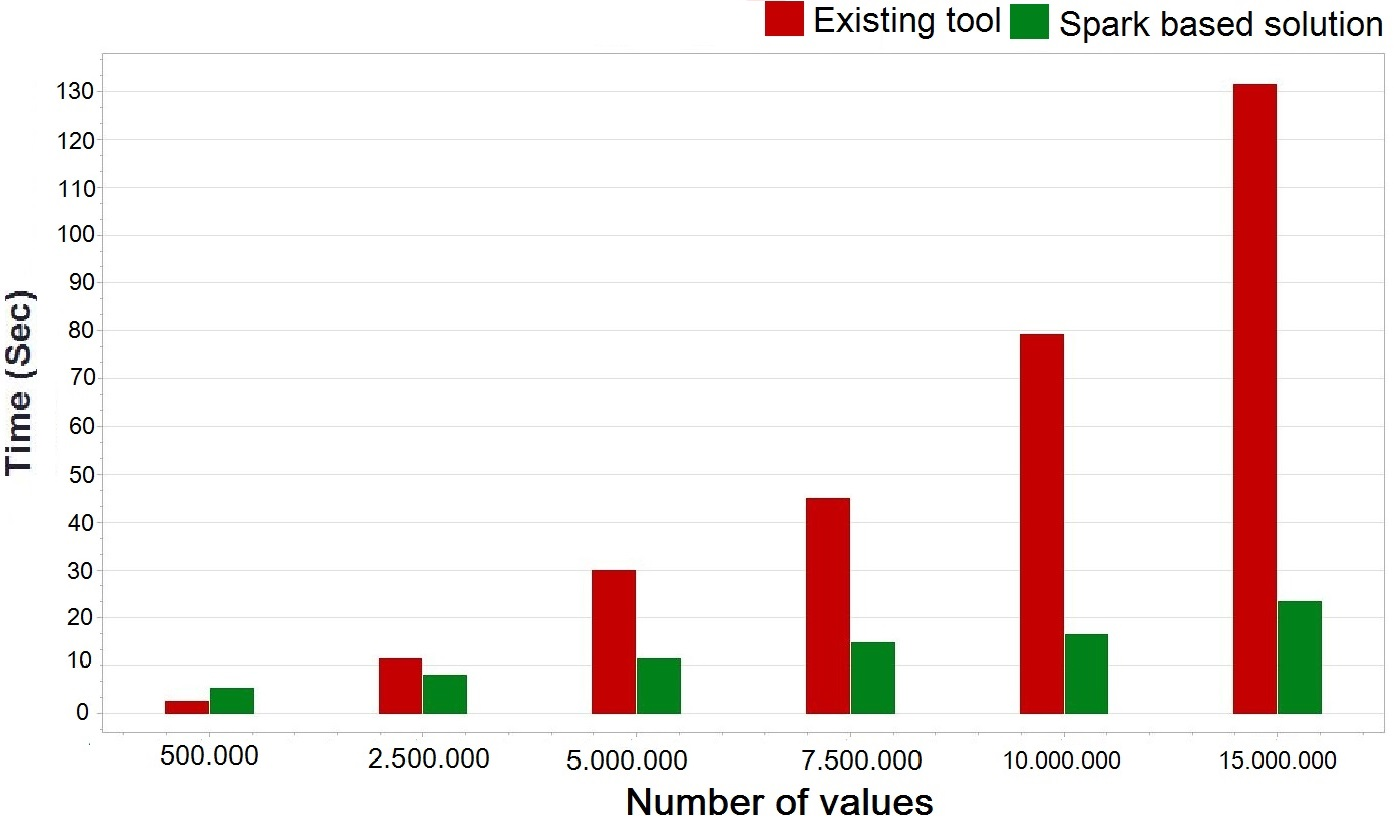
\includegraphics[width=15cm,height=8.5cm]{chapter5/1.JPG}
\end{center}
\caption{Execution Time test}
\label{teste1}
\end{figure}
Figure \ref{teste1} shows the difference between the already used tool and our implemented solution. For a data of 5.000.000 values KnowledgeNet Analytics processes PCA in 29.88 seconds while our solution process it in only 11.49 seconds (more than two times better). The more the data is big the more the difference is bigger. For a data of 15.000.000, KnowledgeNet Analytics takes 2min11s to process PCA while our solution takes 23.45 seconds (5 times better).
\begin{figure}[H]
\begin{center}
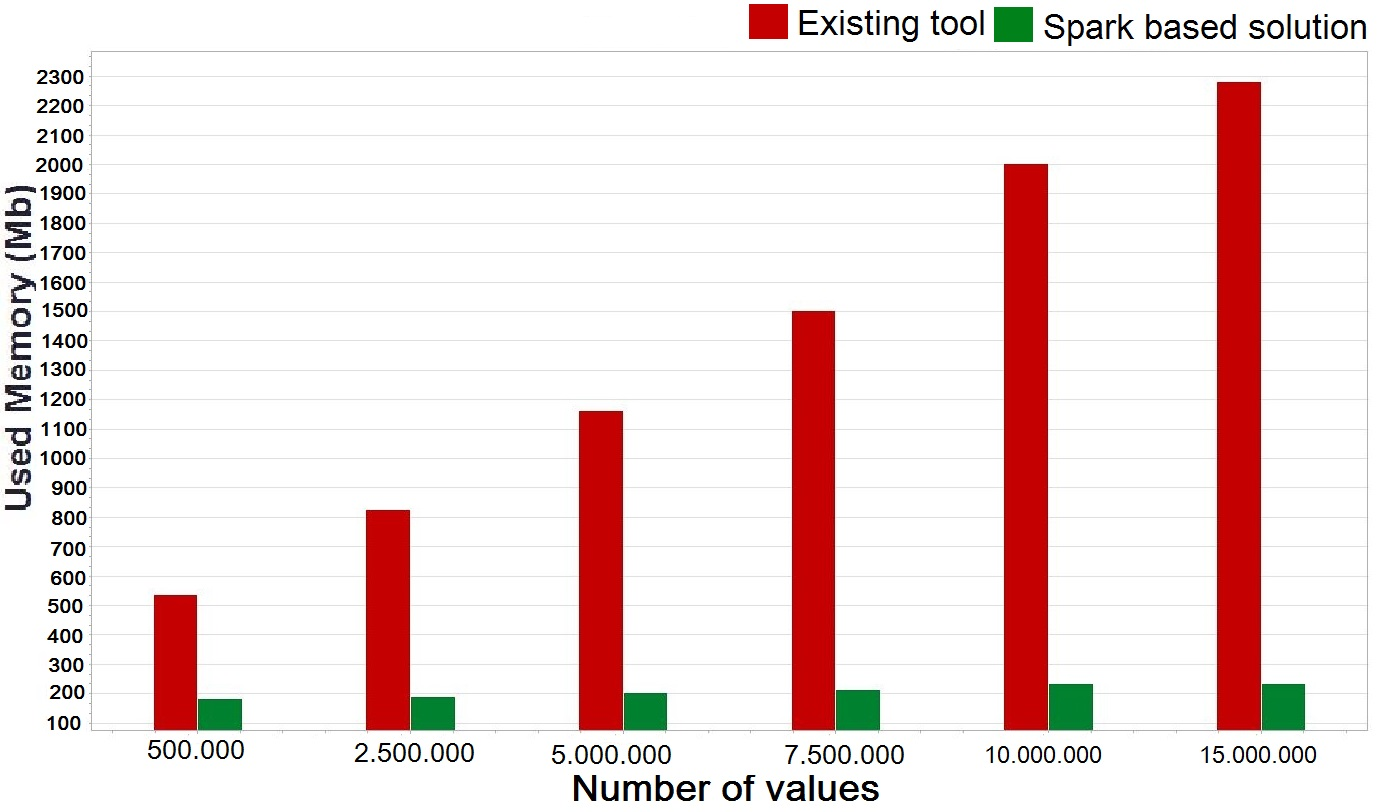
\includegraphics[width=15cm,height=8.5cm]{chapter5/2.JPG}
\end{center}
\caption{Memory Usage test}
\label{teste2}
\end{figure}
Our application doesn't perform execution time only, it also gives great performance in terms of memory usage. Figure \ref{teste2} shows how huge the difference is between KnowledgeNet Analytics and our solution.  For example, data of 5.000.000 values uses 1150 Mb of memory to process PCA algorithm. Our implemented solution takes only 233 Megabytes for more than 15.000.000 values.
\subsubsection{Behavior with Regard to the Number of Nodes}
Figure \ref{nodes} shows our solution behavior in term of run time vs. number of nodes. The used data is about 70 Megabyte of size.
\begin{figure}[H]
\begin{center}
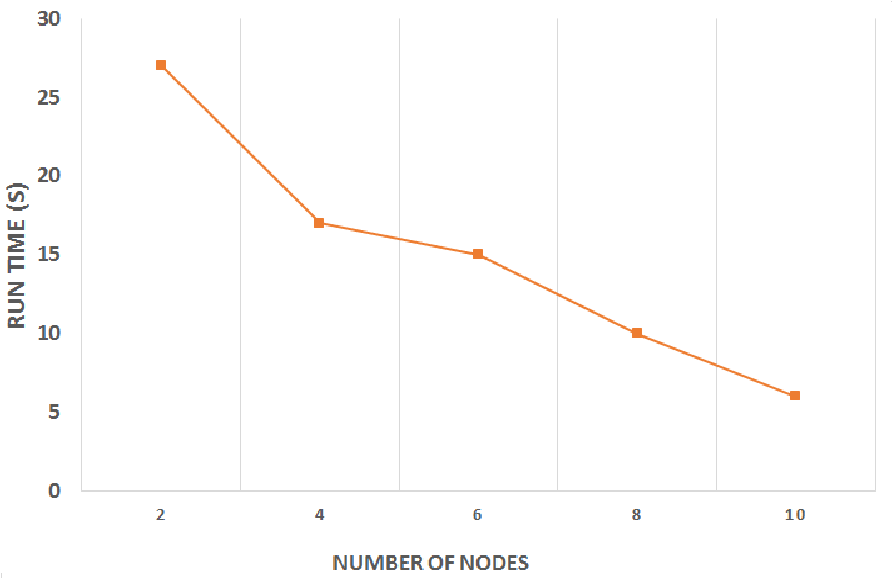
\includegraphics[width=13cm,height=7cm]{chapter5/nodes.png}
\end{center}
\caption{Time Performance Vs. Number of Nodes}
\label{nodes}
\end{figure}
\subsection{Illustrations from the Realization}

Figure \ref{explorer} shows the data explorer provided by our application. It provides all the needed functionalities to users to manage their own data. Thus they can create folders, upload csv files, move their files from one directory to another and many other features.\\

Figure \ref{chartpca} shows the chart loaded from the pca algorithm procced over data from a csv file. Results are shown after users configuration (axes and result file).\\

Figure \ref{chartkmeans} shows kmeans chart loaded. Clusters are represented by colours. Before loading the chart, the user have to fill the configuration form in order to suit the result to his needs.\\

Figure \ref{chartregression} shows linear regression chart. The result is represented with a scatter chart. A step of configuration precede the load of this chart.\\

~\\
~\\
~\\
~\\



\begin{figure}[H]
\begin{center}
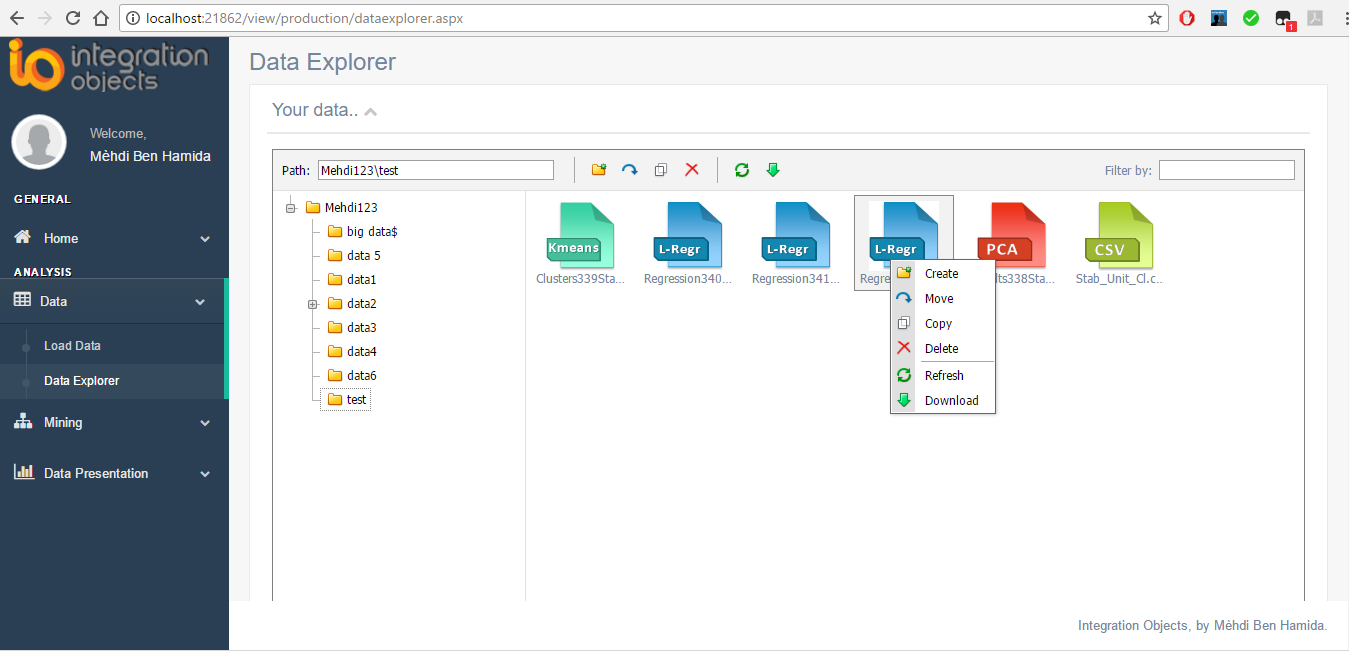
\includegraphics[width=17cm,height=10cm]{chapter5/dataexplorer.png}
\end{center}
\caption{Data File Manger}
\label{explorer}
\end{figure}

\begin{figure}[H]
\begin{center}
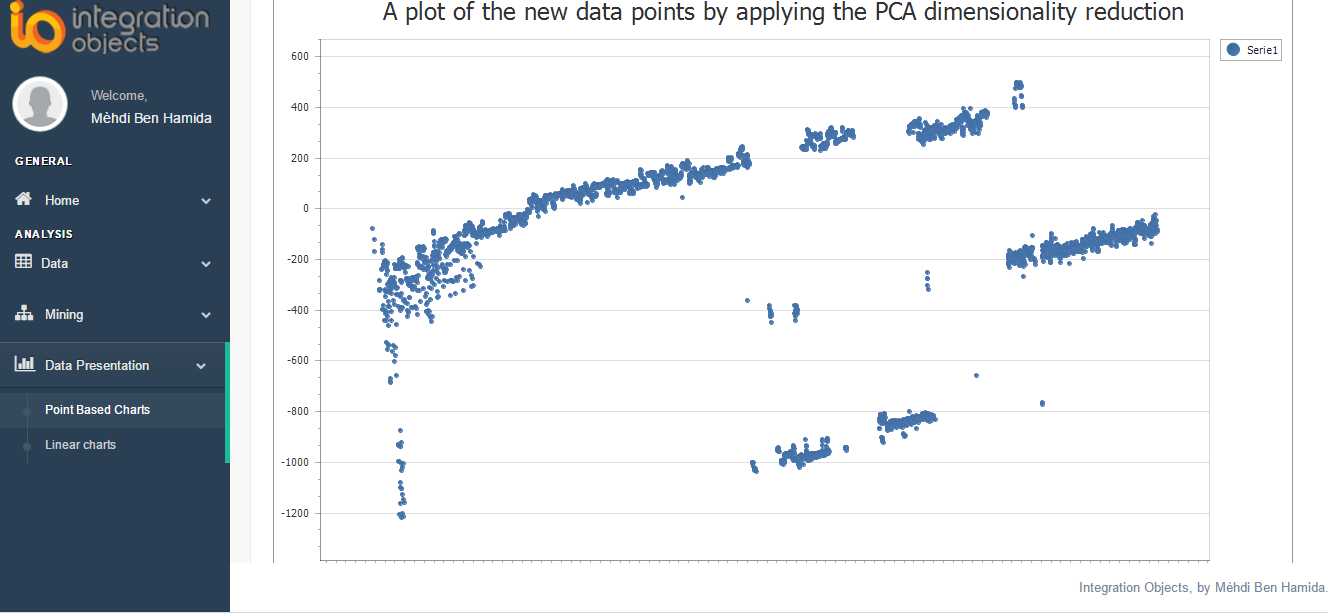
\includegraphics[width=17cm,height=10cm]{chapter5/pca.png}
\end{center}
\caption{PCA Results Chart}
\label{chartpca}
\end{figure}


\begin{figure}[H]
\begin{center}
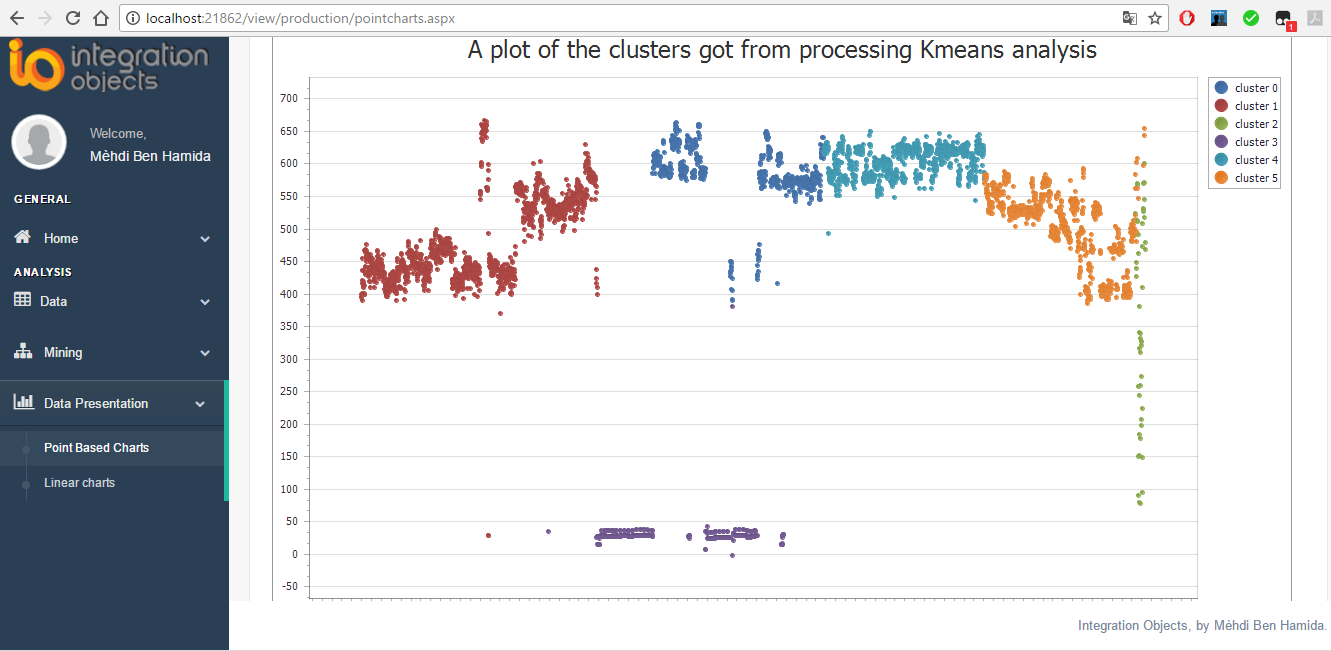
\includegraphics[width=17cm,height=10cm]{chapter5/kmeans.png}
\end{center}
\caption{Kmeans Results Chart}
\label{chartkmeans}
\end{figure}


\begin{figure}[H]
\begin{center}
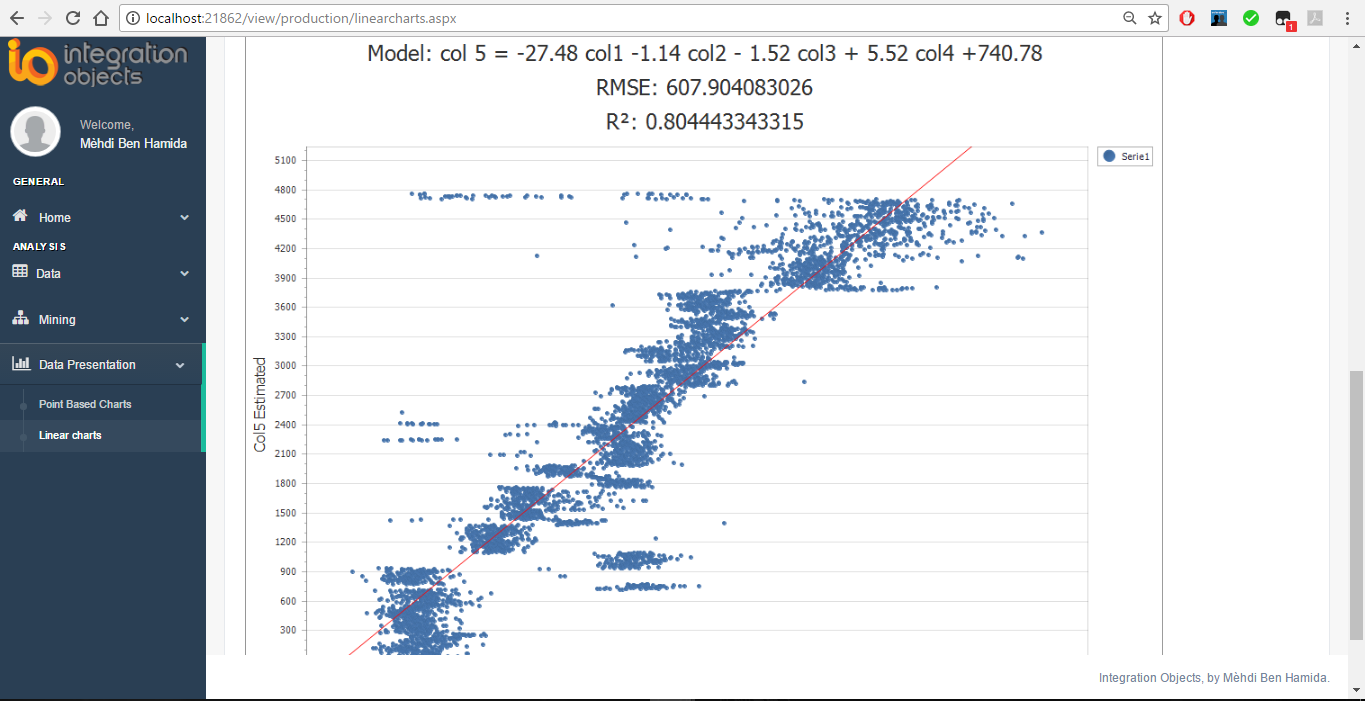
\includegraphics[width=17cm,height=11cm]{chapter5/linear.png}
\end{center}
\caption{Linear Regression Results Chart}
\label{chartregression}
\end{figure}
~\\
After a user launches an algorithm to be processed in the service server, a thread is created to be executed in a console application. Figure \ref{work} shows the background work in progress.\\

\begin{figure}[H]
\begin{center}
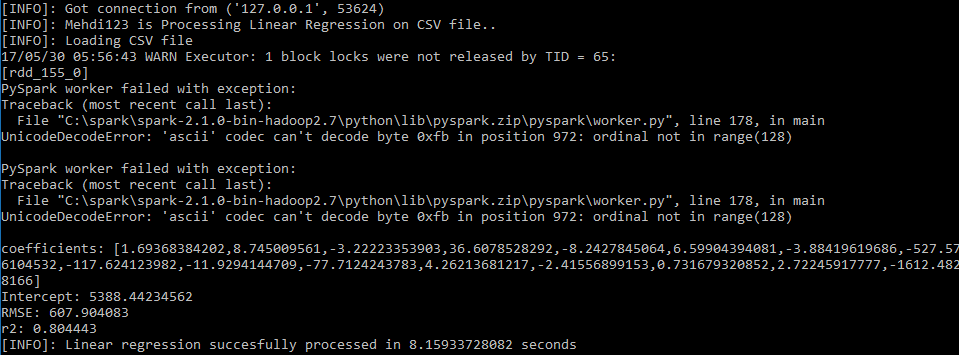
\includegraphics[width=17cm,height=7cm]{chapter5/work.png}
\end{center}
\caption{Background Service Server Execution}
\label{work}
\end{figure}
More achievement captures are represented in appendix \ref{achievement}.
\newpage


\section{Project Timeline}
The project timeline presented in the figure \ref{plan} describes how, we distributed the tasks achievement
during the sixteen weeks starting from February $1^{st}$, to May $31^{th}$.
\begin{figure}[H]
\begin{center}
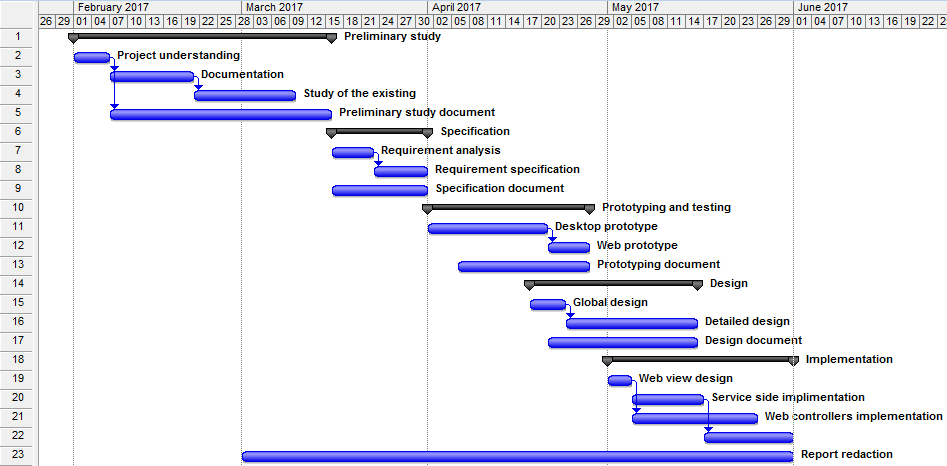
\includegraphics[width=17cm,height=9.7cm]{chapter5/plan.png}
\end{center}
\caption{Project Timeline}
\label{plan}
\end{figure}
\section*{Conclusion}
This final chapter described the implementation phase of our project. First, it presented the tools that we had used during the project life cycle. Then it presented some interfaces offered by our solution, in order to check the correspondence with the requirement specification.